% 34-19(34쪽) — $y=3^{x}$, $y=\left(\dfrac{1}{9}\right)^{x}$ 의 그래프와 선분 $\pt{OP}$(원문 「오른쪽 그림」). 스캔 화질이 낮아 TikZ 로 다시 그림.
% 라벨은 원문 것만: 두 그래프 이름, 두 그래프가 만나는 점 높이의 $1$, 점 $\pt{P}$, $\pt{O}$.
% 점 $\pt{P}$ 의 $x$좌표(답)가 읽히지 않게 $x$축 눈금은 적지 않는다.
\begin{tikzpicture}[line width=0.6pt, x=0.62cm, y=0.44cm, >=stealth]
  \draw[->, line width=0.7pt] (-1.50,0) -- (1.60,0) node[below=1pt] {$x$};
  \draw[->, line width=0.7pt] (0,-0.85) -- (0,4.85) node[left=1pt] {$y$};
  \draw[domain=-1.38:1.25, samples=90, smooth] plot (\x, {pow(3,\x)});
  \draw[domain=-0.62:1.45, samples=90, smooth] plot (\x, {exp(-2.1972*\x)});
  \draw[line width=0.5pt] (0,0) -- (1.0,3.0);
  \fill (1.0,3.0) circle (2.2pt);
  \node[anchor=west, font=\small] at (1.06,3.0) {$\pt{P}$};
  \node[anchor=east, font=\small] at (-0.06,1.0) {$1$};
  \node[anchor=north east, font=\small] at (-0.06,-0.06) {$\pt{O}$};
  \node[anchor=south east, font=\scriptsize] at (-0.64,3.50) {$y=\left(\dfrac{1}{9}\right)^{x}$};
  \node[anchor=south west, font=\scriptsize] at (0.90,3.90) {$y=3^{x}$};
\end{tikzpicture}
